\documentclass[12pt, french, twoside]{report}
%\usepackage[total={6.5in,10in}, top=0.8in, left=1in, includefoot]{geometry}
\usepackage[a4paper, total={6.5in, 10in}, top=0.8in, left=1in,
    headheight=48pt,
    includefoot, includehead]{geometry}
\usepackage{hyperref} % les hyperliens !!!
% \usepackage[utf8]{inputenc}
\usepackage[T1]{fontenc}
\usepackage{mathptmx} %Times font (contraint par le CPBx)
\usepackage{amsmath} % for matrices print
\usepackage{titlesec}
\usepackage{xcolor}
\usepackage{graphicx}
\usepackage{caption}
\usepackage{subcaption}

% Custom chapter design
\titleformat{\chapter}[hang]
  {\normalfont\bfseries\Huge}
  {\thechapter\quad}{0pt}{\Huge}
\titlespacing*{\chapter}{0pt}{0pt}{32pt}

\usepackage{babel, csquotes, xpatch}
%\usepackage{polyglossia}
%\usepackage[backend=biber, style=numeric]{biblatex}
%\addbibresource{biblio.bib}
\usepackage[nottoc]{tocbibind}
\usepackage[square,numbers]{natbib}
\bibliographystyle{plainnat}

\usepackage{amsfonts}
\usepackage{fancyhdr} % Pour la mise en page des en-têtes + pieds de page
\usepackage{lastpage} % pour avoir accès à la dernière page
\usepackage[toc]{glossaries} % glossaire auto, on peut s'y référer dans le latex avec \Gls{maRef}

\makeglossaries

% mettre les éléments du glossaire ici
\newglossaryentry{edit_dist}{
        name={distance d'édition},
        description={C'est le nombre minimal d'opérations (insertion, substitution, suppression) à appliquer à une chaîne de caractères $a$ pour obtenir la chaîne de caractères $b$}
}

\newglossaryentry{api}{
        name={API},
        description={Alphabet Phonétique International.\cite{IPA_handbook}}
}

% Custom header and footer for normal pages
\fancypagestyle{normal}{
  \fancyhf{}
  \fancyhead[RO]{\nouppercase{\hfill\leftmark}}
  \fancyhead[LE]{\nouppercase{\rightmark\hfill}}
  \fancyfoot[L]{Mémoire CPBx}
  \fancyfoot[C]{\thepage/\pageref{LastPage}}
  \fancyfoot[R]{2023}
  \renewcommand{\headrulewidth}{1pt}
}

% Custom header and footer for new chapter pages
\fancypagestyle{newchapter}{
  \fancyhf{}
  \fancyfoot[L]{Mémoire CPBx}
  \fancyfoot[C]{\thepage/\pageref{LastPage}}
  \fancyfoot[R]{2023}
  \renewcommand{\headrulewidth}{0pt}
}

% Set the new chapter page style to the custom style
\pagestyle{normal}
\makeatletter
\let\ps@plain\ps@newchapter
\makeatother

\begin{document}
\begin{titlepage}
    \centering
    \vspace*{\fill}

    \huge\bfseries
    Les utilisations possibles de l'Intelligence Artificielle dans la linguistique historique
    
    \vspace*{1.5cm}
    \large Thomas HORRUT,\; Eliott CAMOU,\; Benjamin BADOUAILLE\\
    Étudiants au Cycle Préparatoire de Bordeaux (CPBx) 

    \vspace*{1.5cm}
    \large Projet tutoré par Rachel Bawden
    \vspace*{1.5cm}

    \begin{figure}[!h]
        \centering
        \begin{subfigure}[b]{0.2\textwidth}
            
\includegraphics[width=\textwidth]{logo/cpbx_logo.png}
        \end{subfigure}\hspace{0,5cm}
        \begin{subfigure}[b]{0.5\textwidth}
            
\includegraphics[width=\textwidth]{logo/univ_bordeaux_logo.png}
        \end{subfigure}
        \begin{subfigure}[b]{0.2\textwidth}
            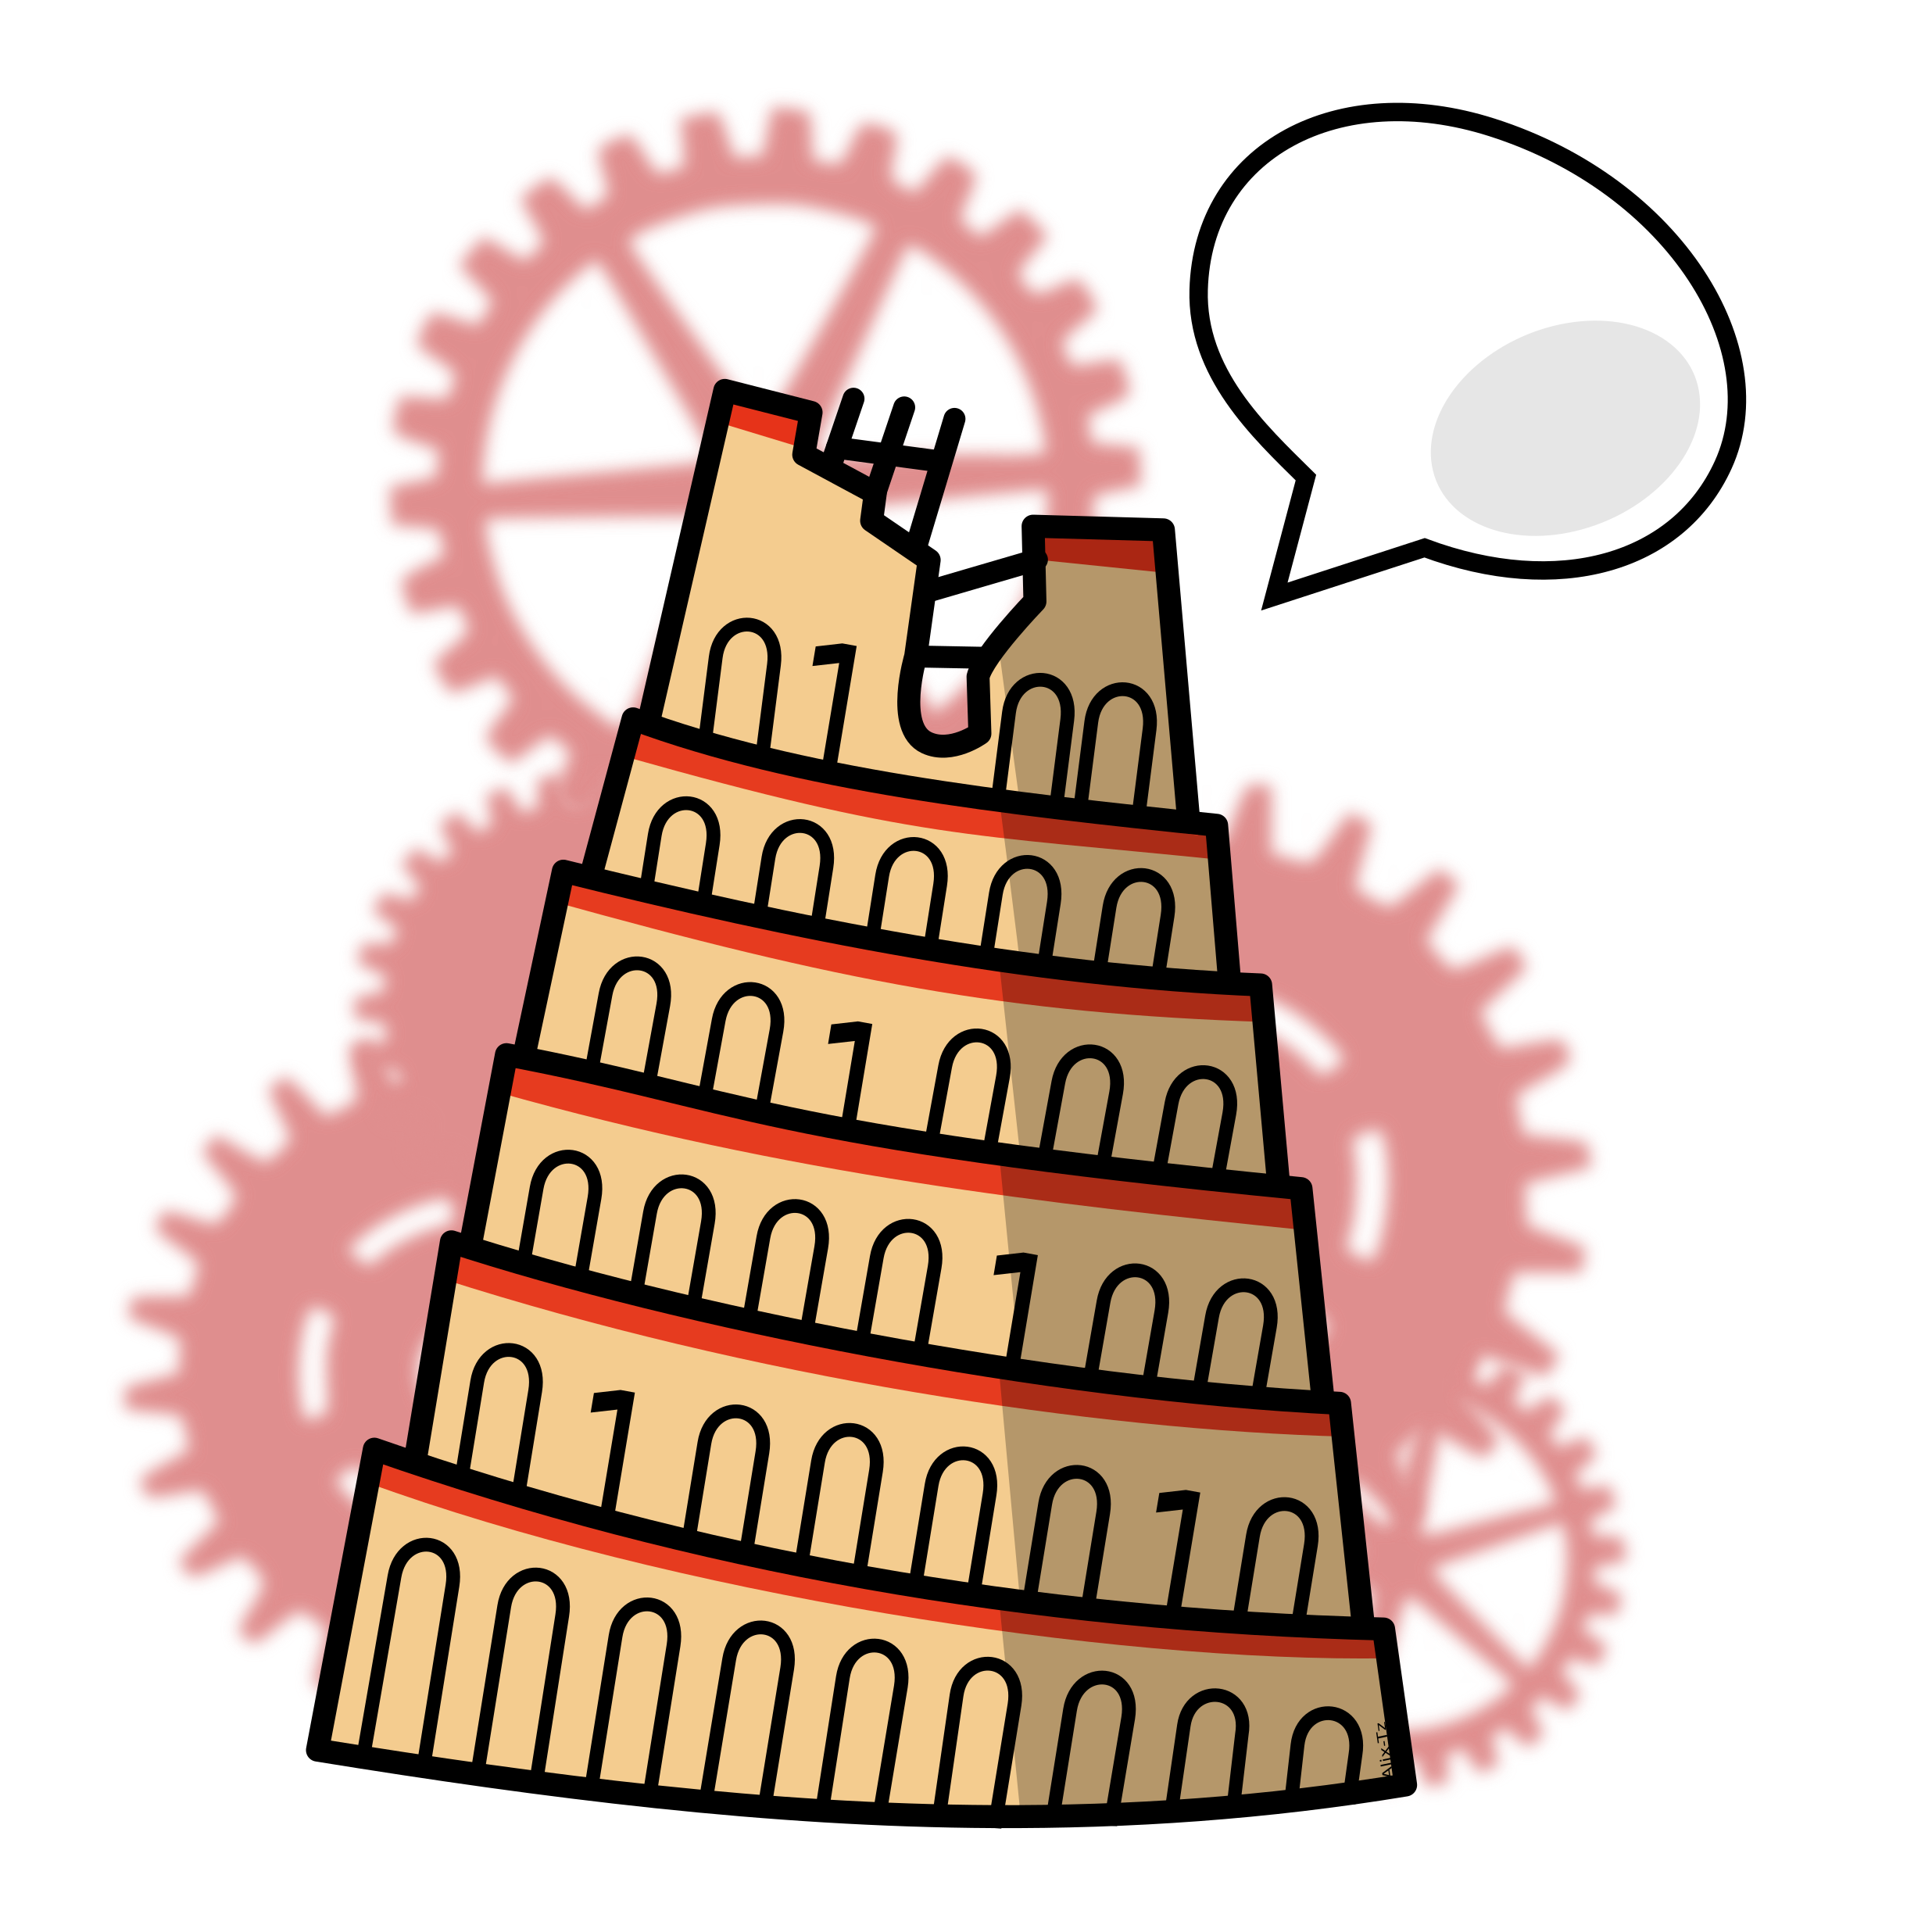
\includegraphics[width=\textwidth]{logo/almanach_logo.png}
        \end{subfigure}
    \end{figure}

    \begin{figure}[!h]
        \centering
        \begin{subfigure}[b]{0.4\textwidth}
            
\includegraphics[width=\textwidth]{logo/logo_enseirb.jpg}
        \end{subfigure}\hspace{1cm}
        \begin{subfigure}[b]{0.4\textwidth}
            
\includegraphics[width=\textwidth]{logo/logo_ensc.jpg}
        \end{subfigure}
    \end{figure}
    
    \vspace*{\fill}
\end{titlepage}

\null
\setcounter{page}{1}
\thispagestyle{empty}
\newpage % Première page blanche pour la numérotation (contrainte de mise en page)
\section{Résumé}
\section{Abstract}
\section{Remerciements}


\tableofcontents
\listoffigures
\listoftables %si inutile, on le virera

\printglossary % TODO: faire marcher ça

\chapter{Introduction}
\textit{Mise en contexte pour arriver à la problématique, quel est le potentiel de l'intelligence artificielle dans la linguistique historique ? ... ?}

\chapter{La linguistique historique et l'Intelligence Artificielle}

\textit{Introduire le but de cette première partie, consitant à familirariser le lecteur à la linguistique historique et l'intelligence artificielle, pour permettre lui permettre de suivre la suite du mémoire.}

\section{La linguistique historique}
\subsection{Introduction à la linguistique historique}

% Remarque plan à retravailler
% L'introdcution à la linguistique "général" jusqu'à arriver à la linguistique historique est bien, mais n'est-il pas toute aussi intéressant d'introduire directement la linguistique historique à la manière de https://www.cairn.info/la-linguistique-jean-perrot--9782130584575-page-59.htm ?
% Ensuite dans la partie "différents principes" -> "différents concepts", introduction au lecteur comme évoqué à l'évolution (l'histoire culturelle) de la langue, à la morphologie (morphème) et la phonétique (phonème), et à la présence de "lois d'évolutions" (ex: régularité phonétique).
% Sur la dernière partie, faire apparaitre la limite des linguistes dans certaines tâches, comme que le déchiffrement de système d'écriture à pris des décennies avec des exemples. Et la capacité d'une machine à pouvoir traiter bcp de données, et à chercher les similarités. Ce processus apportera-t-il une accélération des tâches dans ce domaine ? C'est toute la question de notre mémoire (laisser le suspence).  

La linguistique est la discipline s'intéressant à l'étude du langage. Elle se distingue de la grammaire, dans la mesure où elle n'est pas prescriptive mais descriptive. La linguistique a des rapports très étroits avec d'autres sciences, tout en étant très différente, comme l'ethnographie, ou l'anthropologie. La linguistique peut se définir comme une science qui a pour objet l'étude du langage, des langues envisagées comme systèmes sous leurs aspects phonologiques, syntaxiques, lexicaux et sémantiques.\\

La langue est une partie du langage. C'est un produit social de la faculté du langage et un ensemble de conventions nécessaires, adoptées par une communauté pour permettre l'exercice de cette faculté chez les individus. C'est une institution sociale. Le langage quant à lui est un système de signes qui permet l'expression de la communication.\\

% Appuyer la dimension que la langue est porteur de l'histoire culturelle. L'histoire sociale et de la langue sont indiscossiablement liées. [Comprendre la linguistique, Robert Martin]
% Comprendre une langue par son histoire.
% Introduire ainsi la linguistique historique qui étudie justement la langue sous son aspect historique, en considérant l'évolution de la langue. Elle possède des méthodes qui lui sont propres s'inspirant de l'approche diachronique et des synchronies successives, tout en apportant de la nouveauté (comme les lois d'évolutions).

% Revoir l'introduction de la "linguistique historique"
% Attention à la "principale méthode" ; ne pas résumé la linguistique historique à la reconstruction de langue (ou à la recherche de parenté)
% L'idée d'introduire les lois de variations comme des "lois de proba" est bien, mais un peu tôt, cet aspect sera discuté amplement dans la dernière partie. 
La linguistique historique étudie l'histoire et l'évolution des langues, et des familles des langues. Elle est utilisé, par exemple, dans le déchiffrement de textes anciens, usant de \textit{lois universelles d'évolution}, la tendance de la langue à évoluer suivant certaines \textit{règles}. La principale méthode de travail consiste à une comparaison entre les différents états d'une même langue (synchronie sucessives) ou entre des langues différentes mais issues d'un même ancêtre (comparaison), mais aussi à rechercher des concordances syntaxiques ou sémantiques régulières (loi universelles d'évolution) mettant en évidence la relation entre les différents états d'une langue ou d'un groupe de langues. Par exemple, ce travail de comparaison et de recherche permet de retrouver la langue mère à partir d'une langue fille, comme le latin à partir du français. La linguistique historique permet de caractériser la nature des évolutions, innovations et rétentions l'état initial et les états finaux (phonétique, phonologie, lexique, syntaxe etc.).\\

% Pour raccourcir, on peut enlever cette partie ou la mettre en annexe, si le lecteur souhaite approfondir son histoire.
% La linguistique historique aurait été introduite par Sir William Jones (1746-1794) lorsqu'il émet l'hypothèse que le grec, le latin et le sanskrit auraient des origines communes, menant à une langue Indo-européenne. Une partie de ses hypothèses se seront révélées incorrectes plus tard, mais la langue Proto Indo-Européenne est toujours étudiée aujourd'hui, se voulant être la protoforme du latin, du gothique, du celte, du grec et du perse.\\  
%Si toutes les langues indo-européennes descendent d'une langue primitive commune, quel était donc le peuple qui parlait cette langue, où se situait-il et à quelle époque ? Pour  essayer de répondre à cette question, on se base généralement sur des éléments de linguistique et d'archéologie.\\
%Selon l'hypothèse kourgane, l'indo-européen viendrait d'un peuple semi-nomade ayant vécu il y a environ 6000 à 7000 ans dans la steppe située au nord de la Mer Noire, aux environs de  l'actuelle frontière entre la Russie et l'Ukraine. Dans ce scénario, ce peuple de guerriers et de cavaliers conquérants aurait entrepris de nombreuses migrations, permettant ainsi la diffusion de leur langue en Europe et en Asie.
%Selon l'hypothèse anatolienne, l'indo-européen trouverait son origine en Anatolie (l'actuelle  Turquie) il y a environ 8 à 10 000 ans, à l'époque de l'apparition de l'agriculture dans cette  région. La langue se serait alors répandue dans toute l'Eurasie en même temps que la  diffusion de l'agriculture.
% C'est actuellement l'hypothèse Kourgane qui est considérée comme la plus vraisemblable par les spécialistes, sans cependant être une certitude.

\subsection{Les différents principes} \label{principesLinguistique}

% Approfondir la manière d'aborder la linguistique historique qui ne résume pas qu'à un "mélange" entre de la synchronie et de la diachronie. Ici, ce n'est pas la "linguistique historique" qui peut s'aborder de deux manières mais l'étude d'une langue, en général, qui s'aborde suivant ces manières (qui peuvent s'additionner).
Il existe deux manières d'aborder la linguistique historique : en étudiant une langue à un moment donné, sous un point de vue synchronique, ou en l'étudiant au cours du temps, sous l'angle diachronique. 
% Etudier la proximité d'une langue est l'une des applications de la linguistique historique, mais ne constitue pas un principe en soit. (Plus répétition avec le paragraphe précédent). Sinon bonne idée, de parler de cette application.
% Distinction des emprunts ? Où veux tu en venir ? Proche par "hasard" sur certains points ?
La proximité entre des langues peut traduire une histoire commune.\\
Cependant, il faut distinguer les emprunts à une ou plusieurs autres langues des caractéristiques ancestrales de la langue étudiée. Après avoir fait la distinction, on peut dire que deux langues ayant des caractéristiques voisines descendent d'une langue plus ancienne commune. Par exemple, les langues romanes comme l'espagnol et le français descendent du latin.\\
Ainsi, à partir de ces langues voisines, on peut tenter de reconstruire leur langue ancestrale, la protolangue ou langue mère. Selon plusieurs théories de linguistiques, cette protolangue est hypothétique et elle descendrait elle-même d'une langue plus ancienne encore.
Pour reconstruire cette protolangue, on doit l'étudier sur plusieurs niveaux : la syntaxe, le lexique, la phonologie, la phonétique... De là, on peut aborder un processus récursif : à partir d'un ensemble de protolangues apparentées, on peut reconstruire une protolangue encore plus ancienne, et remonter un arbre généalogique des langues humaines de cette façon.\\
Pour cela, la linguistique historique doit prendre en compte le sens des mots, mais aussi leur représentation essentielle, caractérisée par une suite de sons -- elle-même représentée ensuite par des symboles. Cependant, les mots de deux langues peuvent être proches, par hasard, à cause d'un emprunt, ou d'une évolution commune des langues.\\
% La problématique de l'emprunt peut être sous développé ?

% Faire apparaitre plus tôt pour comprendre, quand il est parlé d'emprunt
Par exemple, \textit{meli} veut dire \textit{miel} en hawaïen et en grec ancien, sans qu'un lien entre les deux langues ne soit établi. \textit{Algorithme}, \textit{girafe}, \textit{orange}, sont des mots français empruntés à l'arabe. Enfin, les mots \textit{main} et \textit{mano} en espagnol ont la même signification et ont une origine commune. On dit alors qu'ils sont des cognats.\\

% Citer la référence à Saussure pour la définition
Un phonème est un élément sonore du langage articulé considéré d'un point de vue physiologique (disposition des organes vocaux) et d'un point de vue acoustique (perception auditive). 
% Quand cela a t il été expliqué ? N'a t on pas supposé une certaine régularité dans l'évolution des langues.
Comme expliqué précédemment, l'évolution des langues se fait de façon plus ou moins régulière, quantifiable, et prévisible. 
% Mieux expliciter correspondances régulières
Ces changements sont appelés correspondances régulières. Les transformations phonologiques qui changent sans exception un phonème $A$ de la langue $1$ en phonème $B$ de la langue $2$ témoignent d'une relation de parenté entre deux langues.\\
\indent Un morphème est quant à lui le plus petit fragment porteur de sens. Il peut être de nature lexical ou grammatical. En parallèle, on le considère également soit comme un thème morphologique, lorsqu'il porte le sens principal du mot, soit comme un affixe, dans le cas d'un préfixe ou d'un suffixe par exemple. Dans \textit{chant-eur}, \textit{jongl-eur}, ou \textit{jou-eur}, le suffixe  \og -eur \fg{} signifie celui qui fait l'action. Ainsi, \og eur \fg{} est un morphème. La Morphologie est le domaine de la linguistique étudiant les morphèmes et leur manière de composer des mots.\\

% Un exemple pour s'imaginer
Les correspondances régulières sont détectées grâce à la méthode comparative. Pour cela, elle considère un ensemble de mots. Les mots doivent alors être apparentés selon leur sens, en prenant en compte les éventuels glissements sémantiques. Après cela, les emprunts doivent être écartés. Enfin, les régularités doivent être cherchées entres les mots et les différentes évolutions qui ont pu conduire des uns aux autres n'ont plus qu'à être inspectées. (rajouter tableaux, texte explication tableaux, sources tableau)\\

% Attention, à ne pas faire, des allers retours entre les différents concepts trop brutaux, sinon le lecteur se perd.
% Que permet-elles ces listes ?
Cependant, si des emprunts ne sont pas détectés, ils vont fausser toute mesure, en conduisant à sous-estimer la profondeur d'un ancêtre commun à plusieurs langues. Pour cela, il existe des listes de mots du lexique simple, pouvant être exploités par les linguistes, comme par exemple les listes de Swadesh (\url{https://en.wiktionary.org/wiki/Appendix:Latin_Swadesh_list}).\\

% Il est intéressant d'évoquer ces domaines, mais pas de les développer.
% Par contre dans la continuité de l'exemple sur la reconstruction de langues, l'introduction à la comparaison de cognat est intéressante. 
Ces listes sont utilisées en glottochronologie et en lexicostatistique, qui sont deux domaines ouverts par Morris Swadesh.\\
\indent La glottochronologie \footnote{La glottochronologie est la méthode de datation des langues proposée par Swadesh, fut comparée à la détermination de l'âge des fossiles à partir de la désintégration radioactive du carbone 14 (elle n'est cependant plus utilisée car sujette à beaucoup d'inexactitudes).}, et la lexicostatistique \footnote{ La lexicostatistique est une méthode utilisée en linguistique comparative et historique pour mesurer la proximité entre différentes langues. Elle se base sur l'analyse statistique des mots partagés entre ces langues, notamment les cognats, c'est-à-dire les mots ayant une origine commune. Cette approche permet d'évaluer le degré de parenté entre deux langues et de reconstituer leur histoire évolutive. En comparant la fréquence des cognats, on peut ainsi déterminer si les langues étudiées sont issues d'une même langue ancestrale. Toutefois, la lexicostatistique présente des limites, notamment en raison de possibles emprunts ou convergences culturelles qui peuvent fausser les résultats.} sont des techniques utilisant les listes de Swadesh. Cependant, bien que ces listes soient toujours utilisées,  ces deux méthodes ont fait place à une application récursive de reconstruction de langue, plus adaptée et tenant compte du contexte sémantique, phonétique et syntaxique des langues.\\ 
% Surement de trop, il faut abbréger.
% \indent Après une reconstruction de ces protolangues, on arrive à regrouper 12 macro-familles de langues :  ces macro-familles sont cependant aussi sujettes à débat. Bien qu'on admette comme très plausible que les proto-langues des familles de langues du monde ont fait partie à leur tour de familles encore plus anciennes, il n'y a pas d'unité de vues concernant la possibilité de reconstruire les proto-langues des superfamilles, parce qu'après une certaine période, les langues changent dans une telle mesure qu'on ne peut plus leur détecter une origine commune. (cf figure) 

% Il n'a pas été démontré cette étude des phonèmes, ainsi, il ne peut y avoir de "donc".
% Cependant, il y a bien eu une étude de la morphologie.
% Pourquoi ne pas présenté, au début, la phonologie et enchainé sur la déf de Saussure. Même raison pour éviter les allers-retours entre les différentes idées.
La phonologie est donc, comme vu précédemment, l'étude des phonèmes. Ces phonèmes ont donc des caractéristiques différentes, se différenciant entre eux de par leur prononciation. 
% Les détails sur la prononciation, et les différents systèmes peuvent être mis en annexe, mais on ne peut détailler cela. Ou bien quelques lignes peuvent être évoqués sur le sujet.
Ainsi, nous allons évoquer quelques notions de phonétique. La phonétique s'appuie principalement sur des caractères physiques qui permettent la prononciation. De nombreux sons peuvent être produits et sont répertoriés dans des tableaux phonétiques \cite{Saussure} (voir image). 
% En Annexe
% Pour la description de l'appareil, nous nous référerons une figure schématique, où $A$ désigne la cavité nasale, $B$ la cavité buccale, $C$ le larynx, contenant la glotte $\varepsilon$ entre les deux cordes vocales.\\
% Dans la bouche on distingue les lèvres $\alpha$ et $a$, la langue $\beta$ - $\gamma$ ($\beta$ désignant la pointe et $\gamma$ tout le reste), les dents supérieures $d$, le palais, comprenant une partie antérieure, osseuse et inerte $f$ et $h$, et une partie postérieure, molle et mobile ou voile du palais $i$, enfin la luette $\delta$.
% Les lettres grecques désignent les organes actifs dans l'articulation, les lettres latines les parties passives. La glotte $\varepsilon$, formée de deux muscles parallèles ou cordes vocales, s'ouvre par leur écartement ou se ferme par leur resserrement. La fermeture complète n'entre pour ainsi dire pas en ligne de compte ; quant à l'ouverture, elle est tantôt large, tantôt étroite. Dans le premier cas, l'air passant librement, les cordes vocales ne vibrent pas ; dans le second, le passage de l'air détermine des vibrations sonores. Il n'y a pas d'autre alternative dans l'émission normale des sons. La cavité nasale est un organe tout à fait immobile ; le passage de l'air peut être arrêté par le relèvement de la luette $\delta$, rien de plus ; c'est une porte ouverte ou fermée.\\

Ainsi, on peut voir que la prononciation des phonèmes et des sons proviennent de parties très variées du corps humain. 
%Nous allons étudier le système phonologique français , qui est composé de 36 phonèmes : $17$ sont dits consonantiques ; ils mettent en jeu les $20$ consonnes de l'alphabet, $16$ sont dits vocaliques ; ils mettent en jeu les $6$ voyelles de l'alphabet et $3$ semi-consonantiques ou semi-vocaliques.\\
% En Annexe
%Phonème consonantique : [ p ] de paon, [ f ] de faon,  [ b ] de banc, [ v ] de vent, [ t ] de temps [ d ] de dent, [ s ] de sans, [ z ] de zan, [ \textesh  ] de chant [ \textyogh  ] de Jean,  [ g ] de gant, [ k ] de quand,  [ l ] de lent, [ \textscr ] de rend,  [ m ] de ment, [ n ] de non,  [ \textltailn ] de pagne
%Phonèmes vocaliques :  [ a ] de patte, [ \oe ] de œuf,  [ ɑ ] de pâte, [ \o ] de feu, [ \~a ] de pente [ o ] de côte, [ \textschwa  ] de petit, [ o ] de cotte, [ e ] de pré, [ \~{\textopeno} ] de conte, [ \varepsilon ] de prêt [ i ] de nid, [ \~{\varepsilon} ] de brin, [ y ] de nu, [ \~{\oe} ] de brun, [ u ] de nous. 
%Phonème semi-consonantique ou semi-vocalique : [w] de oui, [j] maille, [\textturnh] de pluie.\\

Les phonèmes sont susceptibles d'évoluer dans le temps suivant des \og lois phonétiques\fg. De plus, les phonèmes, dans une langue, peuvent apparaître ou disparaître, comme par exemple le /h/ aspiré au 17ème siècle, cette disparition s'étalant jusqu'au 19ème siècle.  L'évolution des phonèmes est due principalement à la loi appelée \og \textit{paresse articulatoire} \fg{} : ce qui est trop difficile à articuler est automatiquement simplifié. C'est ainsi que les mots ont été raccourcis, par disparition des syllabes les plus faibles. Des consonnes se sont affaiblies : placées entre 2 voyelles (intervocaliques), elles ont été influencées, se sont sonorisées, et ont pu disparaître. Ce phénomène aboutit à la longue à de profondes transformations de la morphologie, comme la chute des déclinaisons, et la modification des conjugaisons. (par exemple, "pater" en latin est devenu "père" en français, ou encore par exemple, le \og s\fg{} final de "plus" était autrefois prononcé, mais est devenu muet au fil du temps.\\
\indent Cette loi de simplification est compensée par la loi d'\og \textit{intelligibilité} \fg, la nécessité de clarté dans l'expression : il faut que les mots et les phrases restent compréhensibles ; on a donc conservé certains phonèmes pour éviter que la réduction n'amène des homophones, ou que la phrase devienne obscure. (Par exemple, le son [e] a évolué en “è” ou “ê”, et le son [o] a évolué en “au" ou "eau". De plus, les voyelles suivant une consonne nasale ont tendance à se nasaliser, comme dans le cas de "enfant" où le "a" est nasalisé.)\\ 
Pour terminer avec la phonétique, voici quelques principes qui régissent les modification phonétiques à travers le temps : 
% uniquement citer et rajouter cette partie en annexe
%La palatalisation : La palatalisation est un processus phonétique qui consiste à prononcer une consonne avec un son de palais mou. Par exemple, en ancien français, le son "ch" était prononcé "k" dans certains mots, mais a évolué vers un son de palais mou en français moderne, comme dans le mot "chien".
%La diphtongaison : La diphtongaison est un processus phonétique qui consiste à ajouter un deuxième son vocalique à la fin d'un son vocalique existant. Par exemple, en ancien français, le son "i" dans le mot "pierre" était prononcé comme une voyelle simple, mais a évolué vers un son diphtongué "ie" en français moderne.
%La chute des voyelles : La chute des voyelles est un processus phonétique qui consiste à éliminer une voyelle en position finale ou médiane d'un mot. Par exemple, le mot "femme" était autrefois prononcé avec une voyelle en position médiane, mais cette voyelle est tombée au fil du temps, laissant le mot avec deux consonnes.
%La liaison : La liaison est un processus phonétique qui consiste à lier la dernière consonne d'un mot avec la première voyelle du mot suivant. Par exemple, dans la phrase "les amis", la liaison est faite entre le "s" de "les" et le "a" de "amis".
%La nasale : La nasalisation est un processus phonétique qui consiste à produire un son nasal en passant de l'air par les fosses nasales. Par exemple, en français, les voyelles suivant une consonne nasale, comme le "n" ou le "m", sont nasalisées, comme dans le mot "enfant".\\ 

\subsection{Les atouts de l'Intelligence Artificielle dans ce domaine}
\textit{La linguistique historique fait face à de nombreux problèmes récurrents (traiter une grande quantité de textes pour l'homme, remarquer des motifs dans ces documents historiques). Alors que ce travail pourrait être effectué par une machine, grâce à sa capacité à traiter un grand nombres de données, et à chercher des similarités dans ces données. Avant, de voir les tâches où l'Intelligence Artificielle peut intervenir, il est d'abord nécessaire de voir en détail la conception des ces IA.}

Résoudre des problèmes de Linguistique Historique avec un ordinateur nécessite de lui faire traiter
du contenu textuel devant être abstrait sur des terrains parmi ceux de la \textbf{phonétique}, de la
\textbf{sémantique}, de la \textbf{morphologie} ou encore de la \textbf{syntaxe}.\\
\textbf{\textit{Développper un exemple pour illustrer ces 4 niveaux d'abstractions}}

La réalisation de ces abstractions s'inscrit dans le Traitement Automatique des Langues (TAL),
un domaine à cheval entre la Linguistique et l'Informatique. L'Intelligence Artificielle y occupe
une place centrale pour sa capacité à effectuer des approximations améliorables avec de l'entraînement.
\section{L'intelligence artificielle dans le Traitement Automatique des Langues}
\subsection{Introduction à l'apprentissage automatique}
\textit{Qu'est ce qu'une intelligence artificielle ?\\
    Qu'est ce qu'un réseau de neurones ?\\
    Quel est le principe derrière l'apprentissage automatique ?\\
    Définition des apprentissages supervisés/non supervisés
    Définition de propagation avant.
    Définition rétro-propagation du gradient.
    Exemple de FFNN pour tâche de classification}

Un important nombre de problèmes informatiques peut être résolu à travers la détermination d'une fonction mathématique $f$ d'un espace vectoriel $\mathbb{K}^n$ vers un espace vectoriel $\mathbb{K}^{n'}$ (avec $\mathbb{K}$ correspondant à $\mathbb{R}$ ou $\mathbb{C}$).\\
Lorsqu'un algorithme conventionnel est développé pour réaliser un tâche, $f$ a déjà implicitement été trouvé. Par exemple, derrière un traitement opéré sur une chaîne de caractères, elle existe bien, avec pour entrée une séquence de $n$ caractères encodés sous forme de bits qui forme un vecteur de l'espace $\mathbb{R}^n$ et pour sortie un élément d'un espace $\mathbb{R}^{n'}$ représentant la chaîne de sortie.\\
En revanche, de nombreux cas demeurent où il est difficile -- voire impossible -- de poser une expression mathématique ou un algorithme pour répondre à certains problèmes. On considère alors $f$ comme hypothétique et on cherche à l'approcher à partir d'un \textbf{modèle}, qu'on construit à partir des informations qu'on dispose sur $f$, comme un ensemble de ses points $\{(x_k, y_k=f(x_k)), k \in S\}$, à travers une tâche dite de \textbf{régression}.

\vspace{12pt}
Les \textbf{réseaux de neurones} sont des outils performants pour établir des modèles. Mathématiquement, ce sont des compositions d'applications non-linéaires et linéaires recevant un vecteur d'entrée représentant une donnée et sortant un vecteur de sortie représentant un résultat dans un format cohérent avec le problème.

\subsubsection{Définitions, du neurone au réseau}
Le neurone artificiel le plus élémentaire effectue la \textbf{somme pondérée} des coefficients du vecteur d'entrée, à laquelle il ajoute une valeur de \textbf{biais} pour enfin calculer l'image de la somme à travers une fonction non-linéaire dite \textbf{d'activation}. La sortie du neurone est donc un réel ou un complexe. Si on la note $y_i$, qu'on note $x$ le vecteur d'entrée dans $\mathbb{K}^n$, $w_i$ le vecteur de \textbf{poids} associé au neurone, $b_i$ son biais et $\sigma$ sa fonction d'activation, on a :
\begin{equation}
    y_i = \sigma(b_i + \sum_{j=0}^{n} w_{ij}x_j) = \sigma(b_i + <w_i, x>)
\end{equation}\cite[section 1]{jurafsky_ffnn}

Une \textbf{couche de neurones} est la mise en commun d'un nombre abritraire $N$ de neurones devant prédire des sorties $y_i$ différentes. Leurs vecteurs de poids $w_i$ diffèreront donc. En revanche, leur fonction d'activation est identique. La sortie d'une couche est donc un vecteur $y$ pouvant s'écrire comme dans l'équation \ref{def_couche}\footnote{On y confond la fonction d'activation avec la fonction vectorielle $\sigma$ s'appliquant indépendamment à chaque coefficient.}.
% Il n'est pas très correct visuellement d'effectuer cette approximation. Tout le but de ces fonctions d'activation est de permettre cette non linéarité (sinon peut importe le nombre de couches au réseau, si toute les neurones sont linéaires, alors elle se résumeront à un espace linéaire par combinaison linéaire. Jurasky). Il est peut être plus simple d'évoquer uniquement que'une couche de neurones n'est qu'un ensemble de neurones.

\begin{equation} \label{def_couche}
    \begin{split}
        y & =
        \left(\begin{matrix}
            \sigma(b_1 + <w_1, x>) \\
            \sigma(b_2 + <w_2, x>) \\
            \vdots \\
            \sigma(b_i + <w_i, x>) \\
            \vdots \\
            \sigma(b_N + <w_N, x>)
        \end{matrix}\right)
        =
        \sigma\left(\begin{matrix}
            b_1 + \sum_{j=0}^{n} w_{1j}x_j \\
            b_2 + \sum_{j=0}^{n} w_{2j}x_j \\
            \vdots \\
            b_i + \sum_{j=0}^{n} w_{ij}x_j \\
            \vdots \\
            b_N + \sum_{j=0}^{n} w_{Nj}x_j
        \end{matrix}\right)\\
        & = \sigma\left(
            \left(\begin{matrix}
                b_1 \\ b_2 \\ \vdots \\ b_i \\ \vdots \\ b_N
            \end{matrix}\right)
            +
            \left(\begin{matrix}
                w_{11} & w_{12} & \hdots & w_{1j} & \hdots & w_{1n} \\
                w_{21} & w_{22} & \hdots & w_{2j} & \hdots & w_{2n} \\
                \vdots & \vdots & \ddots & \vdots & \ddots & \vdots \\
                w_{i1} & w_{i2} & \hdots & w_{ij} & \hdots & w_{in} \\
                \vdots & \vdots & \ddots & \vdots & \ddots & \vdots \\
                w_{N1} & w_{N2} & \hdots & w_{Nj} & \hdots & w_{Nn} \\
            \end{matrix}\right)
            \left(\begin{matrix}
                x_1 \\ x_2 \\ \vdots \\ x_j \\ \vdots \\ x_n
            \end{matrix}\right)
        \right)
        = \sigma(b + Wx)
    \end{split}
\end{equation}

Un réseau neuronal est ainsi formé à partir de la mobilisation d'une ou plusieurs couches. L'intuition derrière l'utilisation de couches intermédiaires, qu'on nomme des \textbf{couches cachées}, est que la machine puisse être capable d'apprendre à construire des \textbf{représentations adéquates} des données pour effecuter la prédiction finalement voulue avec pertinence. On parle alors d'\textbf{apprentissage profond} et cette technique offre des réponses face aux difficultés d'abstraction soulevées par les problèmes de TAL.
% un exemple de problème de TAL ? Le lecteur n'est pas encore complétement familier avec ce concept.

L'agencement des couches et la manière de calculer la sortie finale à partir de chacune d'elles, qu'on peut rassembler sous le terme de \og mode de \textbf{propagation} \fg, est un \textbf{paramètre architecturale} à part entière qu'il faut judicieusement définir en fonction de la tâche à réaliser. Pour traiter de l'utilisation de l'IA dans le TAL, au moins deux principaux types de réseaux de neurones seront introduits au cours de ce chapitre, différant par la nature cyclique ou non de l'enchaînement de leurs couches internes.\cite[introduction + section 3]{jurafsky_ffnn} [\textit{ajouter illustration}]
% Parfait !

\subsubsection{Processus d'apprentissage}
% Exprimer le but de l'entrainement, qu'est que cela permet ? A chaque itération ?
L'entraînement d'un réseau de neurones s'effectue à travers des \textbf{ajustements des poids et des biais dans chaque couche}, dans le cadre d'une \textbf{minimisation d'une fonction de perte}\footnote{aussi appelée fonction de coût, ou d'erreur}. Cette fonction doit être choisie judicieusement selon le problème puisqu'elle exprime l'écart entre les sorties prédites et les sorties ciblées au passage de données d'entrée d'entraînement. Sa minimisation est réalisée par un algorithme de \textbf{descente du gradient}, avec le gradient de la fonction de perte selon tous les poids du réseau qui est calculé grâce à un procédé de \textbf{rétropropagation de l'erreur}, une adaptation pour les réseaux de neurones de celui de la discrimination rétropropagative pour des graphes d'exécution quelconques. Plusieurs implémentations de cet algorithme, qu'on nomme des \textbf{optimiseurs}\footnote{Adam\cite{kingma2017adam} en est un assez connu et est celui qui était prévu d'être utilisé pour le codage de l'expérience.}, existent et la nature de l'optimiseur dans un modèle fait partie de ses paramètres d'entraînement.
% Petit graphique, exemple, pour s'imaginer le processus qui introduit bcp de nouveautés.

% Qu'est qu'un hyperparamètre ?
Des hyperparamètres pour l'entraînement sont également amenés à être définis en pratique, tels que le \textbf{taux d'apprentissage}, fixant la valeur maximale de variation qu'un poids ou biais peut subir au cours d'une rétropropagation, le nombre d'\textbf{époques} (\textit{epochs}), i.e. de balayages de l'ensemble des données du set d'entraînement pour l'exécution des descentes, et enfin la taille des \textbf{lots (\textit{batchs})}, i.e. des groupes de données d'entraînement à envoyer au modèle en une fois\footnote{Cette quantité est pensée pour prévenir les problèmes de saturation de la mémoire des ordinateurs, qui sont favorisés par les ordres de grandeur souvent importante des tailles des jeux de données d'entraînement.}.\cite[17-23]{jurafsky_ffnn}.\cite[21]{fourrier}

% Attention il n'est pas nécessaire d'initialiser aléatoirement les poids, cela peut ausssi s'effectuer de façon pseudo-aléatoire, de façon calculé
\textit{ajouter la nécessité d'initialiser aléatoirement les poids}

\subsubsection{Concevoir correctement}

\textit{
    La phase d'entraînement du réseau s'arrête lorsque le gradient cesse de décroître.\\
    Les hyperparamètres ainsi que certains paramètres architecturaux (nombre de couches, leur dimension) ont le mérite d'être réglés dans des configurations différentes afin de s'assurer d'une convergence optimale du gradient (qui des fois n'arrive pas ; cf. overfitting + vanishing gradient -> évoquer plus tard pour introduire les LSTM)\\
    \\
    La phase d'évaluation du modèle se fait à partir de comparaisons des résultats sortis avec des résultats ciblés pour un set de données dit d'évaluation. Plus particulièrement en TAL, on cherche à trouver des exemples afin de déterminer les cas qu'il a su apprendre à correctement gérer ou non.\\
    On peut également établir des métriques pour quantifier le taux de pertinence du modèle.
    Par exemple la \gls{edit_dist} entre les mots sortis et les mots ciblés, dans le cas de la prédiction de mots.\\
    \\
    Quoiqu'il en soit, le choix de tous les paramètres se fait expérimentalement, à partir d'intuitions basées sur des observations lors de travaux antérieurs sur de la conception de réseaux. Pas de démonstrations mathématiques (que statistiques).\\
    Transition vers la section suivante
    }

\subsubsection{Présentation du FFNN pour une tâche de classification}
\textit{introduire le réseau FFNN\\
    fonction d'activation softmax à la fin\\
    entropie croisée pour la fonction de perte\\
    }
\subsection{Traitement des données}

Avant de donner à un réseau de neurones des données au format quelconque, que ce soit pour son entraînement ou pour réaliser des inférences dessus, il est nécessaire de les pré-traiter. Le but est de les rendre correctes et compréhensibles pour l'intelligence artificielle. Leur transformation se fait selon le type de tâche souhaitée. Néanmoins, dans sa généralité, les étapes de préparation des données en TAL restent les mêmes.\\

% \footnote{À noter que nous parlons ici de \og grandes \fg{} quantités de données à analyser, mais ce mot est relatif à un être humain, et encore, il arrive que ce nombre soit restreint, seulement, pour une IA c'est le contraire, nous parlerons plutôt de d'IA à \og basses ressources \fg{} car ce nombre de données est très petits face à ce qu'elle peut gérer dans le monde moderne et la quantités de textes disponibles sur la toile.}
%[lib nltk] pour segmenter et normaliser
\subsubsection{Normalisation}
Tout d'abord, il faut normaliser (nettoyer) la base de données qui peut être, par exemple, un corpus de textes, une liste de mots, provenant de la toile, ou d'un système de transcription audio-visuelle. Dans ces données se trouvent des chaînes de caractères sous un certains format, où de la ponctuation peut apparaître, de même que des lettres en capitale, des chiffres, des caractères spéciaux (comme le dièse que l'on retrouve souvent dans les \textit{tweets})\dots Mais une partie de ces éléments peut ne pas avoir d'intérêt à être traitée par les algorithmes et même apporter du bruit en fournissant des données incorrectes pour entraîner l'intelligence artificielle. Une première étape est donc de s'en débarasser ou bien d'apporter des modifications à l'aide d'algorithmes de traitement de texte classique\footnote{les Expressions Régulières sont par exemple de puissants outils pour modifier le contenu textuel}.\cite{jurafsky_regular} [Exemple]\\

\subsubsection{Tokenisation}
Après avoir nettoyé la base de données, il faut définir une segmentation des textes en éléments d'entrée pertinents pour un traitement par l'IA : les \textit{tokens}. La tokenisation correspond à la segmentation de chaînes de caractères (comme notre texte) en tokens (mots, sous-mots, caractères, ponctuations). L'ensemble des tokens uniques d'un texte se nomme : vocabulaire.\\
% Nous pourrions discuter longuement de ce qui devrait être pris comme tokens ou non. Par exemple, si nous devons prendre en compte la ponctuation en tant que token. Mais aussi les clitiques si elles doivent être pris en compte, ou si elles doivent être développées. Pour cela, nous vous renvoyons au Chapitre 2 de \og Speech and Language Processing \fg{} de Jurasky.
% Il est intéressant d'évoquer que suivant les différents niveaux de tokenisations (partant du caractères, au sous-mots, jusqu'au mots entier) aide à mieux respectivement à comprendre la morphologie, la sémantique (suivant les sous-mots des algorithmes statistiques), et la syntaxe (suivant les sous-mots basé sur les règles). Et il a été montré qu'il était suffisant de segmenter des phrases en sous-mots pour analyser le langage de manière pertinente. (Thèse Fourrier)
% Résumer la tokenisation sans passer par toutes ces étapes, aller à l'essentiel.
\indent Prenons un exemple \og J'aime les bananes\fg, une approche naïve est de tokeniser notre texte suivant les espaces \footnote{Vous remarquerez déjà que ce processus ne s'applique pas aux langues, comme le Japonais ou le Chinois, manquant d'espace entre les caractères.} ce qui nous donne les tokens [\og J'aime \fg, \og les \fg, \og bananes. \fg] avec un vocabulaire de taille 3 (dans cette phrase tout les tokens sont uniques). Cependant, cette approche pose des problèmes, en commençant par le token \og bananes. \fg{} qui a la même signification avec ou sans point, mais qui sera considéré comme différent pour une IA. Nous pourrions ajouter la séparation suivant la ponctuation, mais alors nous obtiendrons pour \og J'aime \fg{} les tokens [\og J \fg, \og ' \fg, \og aime \fg] qui est une forme tout aussi problématique. Et il existe encore de nombreux cas (les abréviations, les points de suspension, etc.) où ce type de tokenisation pose problème. Une approche alternative est de tokeniser suivant des règles définis, par exemple, de prendre en compte les contractions comme \og J'aime \fg{} et de le transformer en deux tokens [\og Je \fg, \og aime \fg], qui est une méthode beaucoup plus efficace que la première approche, mais montrera des limites face à des situations (ou mots) rares, ou alors il faudrait spécifier de nouvelles règles pour gérer ces cas. Ainsi, la solution proposée est une approche statistique, consistant à décomposer de plus en plus un mot en sous-mots \footnote{Remarquez que le terme \textit{mot} a un sens différent de celui qui le précède.} au fil que sa fréquence diminue. [Exemple].\\
% Intéressant pour la littérature, mais peut être éviter l'exaustivité
\indent Les quatres algorithmes de tokenisation en sous-mots les plus utilisées sont le \textit{Byte-Pair Encoding} (Sennrich et al., 2016), l'\textit{unigram language modeling} (Kudo, 2018), le \textit{WordPiece} (Schuster et Nakajima, 2012), et le \textit{SentencePiece}\footnote{Cet algorithme est une implémentation des deux premiers.} (Kudo et Richardson, 2018).\cite{jurafsky_regular}\\

\subsubsection{Encodage}
Pour la tâche de classification, vous avez vu que les mots d'entrées, [exemple], étaient convertis en une liste de nombre, autrement dit un vecteur, sur lequel il a été effectué des calculs afin d'obtenir un résultat (un nouveau vecteur), [exemple]. Une machine, un réseau de neurones, ne comprend que des nombres et ne sait procéder qu'à des calculs. Il existe différentes façons de convertir un token en un vecteur numérique, mais on retiendra deux méthodes l'encodage 1 parmi n et le plongement lexical (respectivement et plus communément appelés en anglais le \textit{one-hot encoding} et le \textit{word embedding}).\\

L'encodage 1 parmi n consiste à créer un vecteur binaire de la taille du vocabulaire $|V|$, c'est-à-dire, que chaque dimension correspond à un mot dans le vocabulaire. Dans ce vecteur binaire, la valeur est 1 pour la dimension correspondant au mot dans le vocabulaire, et 0 pour toutes les autres dimensions. Ainsi, en supposant que la dimension du mot \og bananes\fg{} se trouve à la troisième dimension (c'est le troisième mot de notre vocabulaire $V$), sa représentation correspondra à un 1 à la troisième dimension du vecteur et à des 0 sur les autres dimensions, soit le vecteur :
\begin{align*}
    \begin{bmatrix}
    0 & 0 & 1 & 0 & \dots & 0
    \end{bmatrix}\\
    \begin{matrix}
    1 & 2 & 3 & 4 & \dots & |V|
    \end{matrix}
\end{align*}
\hfill \cite[(Chap 7, Jurasky)]{jurafsky_ffnn}\\

Comme vous pouvez le voir l'avantage de cet encodage est sa simplicité de mise en oeuvre. Mais le problème survient quand le vocabulaire devient très grand, les vecteurs générés, par définition, deviennent à leurs tours très grands et très dispersés (beaucoup de 0 et peu de 1), ce qui entraine une augmentation de la complexité du modèle (le nombre de dimension pour décrire les données) et des temps de calcul. De plus, cet encodage ne prend pas en compte les relations sémantiques entre les mots, la similarité entre deux mots ne peut être mesuré,  car ils sont encodés de façon indépendante les uns des autres, ce qui peut être particulièrement problématique pour les nombreuses tâches de TAL tel que la compréhension ou traduction d'une langue.\\

Le plongement lexical, en revanche, permet de représenter les mots en encapsulant leur \textit{sens sémantique} par des vecteurs denses de plus faibles dimensions, c'est à dire des vecteurs de nombres réels de petites tailles. Pour obtenir le plongement des tokens, c'est-à-dire, transformer des tokens en vecteurs, une matrice de plongement lexical est utilisée, obtenus par l'entrainement d'un modèle\footnote{Ces modèlent apprenent généralement, de façon non supervisé à partir d'un grand corpus de texte, les relations sémantiques et syntaxiques qui peuvent exister entre les mots. Nous pouvons citer, comme exemple de modèle, Word2Vec, GloVe, Bert, qui sont souvent utilisés pour créer des matrices de plongement lexical. Pour approfondir l'obtention de ces matrices, nous vous invitons à regarder \cite{jurafsky_vector}\cite{jurafsky_ffnn}\cite{jurafsky_11}}. Cette matrice contient, à chaque ligne, le vecteur de plongement lexical d'un token du vocabulaire, et à chaque colonne correspond une dimension du vecteur de plongement. Par ailleurs, les dimensions de ces vecteurs n'ont pas une représentation claire \cite{jurafsky_vector}. Cette matrice représente un espace vectoriel contenant les plongements des tokens d'un vocabulaire, ainsi, les propriétés vectoriels peuvent s'appliquer pour nos tokens vectorisés. Par exemple, étudier la similarité entre deux mots revient à calculer la distance entre les deux vecteurs correspondants, ou encore comme la figure X le montre, les vecteurs peuvent s'additionner/se soustraire permettant d'obtenir un nouveau vecteur qui garde une cohérence sémantique face à ces opérations. [Figure : Exemple de vecteurs sémantiques montrant bien qu'ils portent un sens et permettent des relations sémantiques entre eux ; vecteur "king" $-$ "man" $+$ "women" $->$ "queen"].

% Ignorer l'étape ci-dessous
% Data splitting and batching

\subsection{Architectures neuronales utiles au TAL}
\textit{Quels sont les différents outils ?}

En TAL, le besoin de pouvoir faire comprendre à l'IA des informations \textbf{contextuelles} s'est fait ressentir. Par exemple, pour étudier la langue sur le plan syntaxique, une tâche usuelle est d'attribuer à chaque mot d'une phrase sa nature grammaticale (\textit{part-of-speech tagging}). La phrase est alors une \textbf{séquence} de \textit{tokens} d'entrée qui sont ici des mots. On représente chacun d'eux par un \textit{embedding} ou un vecteur one-hot. Une bonne intuition est celle que des représentations calculées en profondeur dans un réseau de neurones pour certains éléments de la séquence seront utiles pour le calcul de prédictions sur d'autres éléments de cette même séquence. De cette manière, dans la phrase \og La fin de ce film n'était pas très convaincante. \fg{} et dans la phrase \og Ce paragraphe n'est pas bien fin. \fg, ce ne peut être qu'à partir de traitements sur l'ensemble de la séquence de mots qu'un modèle d'IA pourrait correctement sortir que le mot \og fin \fg{}  est tantôt un nom, tantôt un adjectif.

Dans cette section, des types d'architectures vont être présentés pour leur capacité à construire de manière puissante des contextes dans des séquences d'information.
\subsubsection{Réseaux de neurones récurrents}

Grâce à leur architecture cyclique, les Réseaux de Neurones Récurrents (\textit{Recurrent Neural Networks}(RNN)) permettent de prendre en compte un contexte. Étant donné une séquence de $n$ entrées $(x_i)_{1\leq i \leq n}$, le RNN le plus élémentaire est un enchaînement, comme dans un FFNN, d'une couche cachée avec une autre couche. La sortie est alors inférée avec l'expression :
\begin{equation}
    y_i = \sigma(Vh_i)
\end{equation}\footnote{Dorénavant, les vecteurs des biais seront gardés implicites dans les expressions afin de les simplifier.}
La valeur ajoutée du RNN réside dans le calcul de cette couche cachée, qui en plus d'être une fonction de l'entrée $x_i$ de la séquence est également une fonction de la couche cachée qui a été calculée en ayant passé en revue les éléments précédents de la séquence. Une somme pondérée des deux vecteurs est alors effectuée dans la définition de $h_i$, ce pourquoi deux matrices de poids interviennent :
\begin{equation}
    h_i = \sigma'(Hh_{i-1} + Wx_i)
\end{equation}

La propagation du flux d'informations amenant à la sortie d'un modèle RNN pour un certain élément d'une séquence d'entrée peut être illustrée avec le figuré ci-dessous:

\textit{[insérer l'illustration]}\cite[1-4]{jurafsky_rnn-lstm}

De cette façon, on remarque aisément qu'on peut construire des empilements de couches RNN, de la même manière qu'on approfondit l'apprentissage en empilant des couches FFNN. La structure serait semblable à celle présentée ci-dessous:

\textit{[figuré montrant comment l'information + le contexte se propage à travers des empilements de couches RNN]}

Dans ces schémas, la séquence d'entrées n'a été parcourue que de gauche à droite, mais il existe des problèmes, comme celui mentionné en introduction de cette section, où le contexte à gauche comme à droite d'un élément de la séquence doit être pris en compte. Une configuration architecturale des RNNs peut permettre de construire des contextes de manière \textit{bidirectionnelle}. Dans celle-ci, la couche cachée pour l'entrée $x_i$ est produite à partir de la concaténation des couches cachées ayant balayée respectivement les entrées $(x_1, x_2, ..., x_{i-1}, x_{i})$ et dans l'autre sens les entrées $(x_n, x_{n-1}, .., x_{i+1}, x_i)$.

\textit{[Illustrer avec un schéma]}\cite[11-13]{jurafsky_rnn-lstm}

\vspace{12pt}
Pour un RNN simple, 3 matrices de poids doivent donc être entraînées (en plus des biais dans chaque couche). En étalant le graphe des connexions inter-couches pour chaque traitement le long d'une séquence de données d'une certaine taille, comme illustré dans le figuré ??, il est possible d'effectuer une rétropropagation similaire à celle avec les FFNNs pour calculer les dérivées partielles de la fonction de perte selon chaque poids de ces 3 matrices.\cite[4, 5]{jurafsky_rnn-lstm}

En revanche, il a été observé que la descente de gradient ne se déroule pas correctement pour des séquences de taille trop importante, ce qui empêche les simples RNNs d'exploiter efficacement une information contextuelle se situant au-delà d'un certain voisinage autour du \textit{token} à traiter.\cite[25-26]{fourrier}

\subsubsection{Architecture \textit{Long Short-Term Memory}}

Les \textit{Long Short-Term Memories} sont des modèles neuronaux dont l'architecture est une variante à celle des RNNs, conçue expréssemment pour repousser les limitations de ces derniers. Pour cela, il faut entraîner le réseau de neurones à focaliser son \textbf{attention} sur les bons éléments de contexte.

Une unité LSTM est de ce fait plus complexe qu'une unité RNN, mais elle bénéficie de la même modularité. Ainsi, on peut empiler des LSTMs et construire des LSTMs bidirectionnels de la même manière que décrite plus tôt avec les RNNs.\\

La complexification architecturale peut dans un premier temps se remarquer d'un point de vue externe en notant que, là où une unité RNN n'est composée que d'une couche cachée qui est une fonction de l'entrée et de la couches cachée périphérique, l'unité LSTM est composée en plus d'une \textbf{couche de contexte} qu'elle renvoie et qui est utilisée pour le calcul des couches cachées et de contexte des autres entrées dans la séquence.

D'un point de vue interne, ces deux couches interagissent à travers des \textbf{portes} rejettant et promouvant de l'information.

\textit{[Expliquer comment les portes permettent de sélectionner l'information contextuelle + transition]}

\subsubsection{Transformeurs} \label{transformers}

Précédemment, avec les RNN et les LTSM, nous avons introduit le mécanisme d'attention, permettant au réseau de se focaliser sur la manière dont les mots (éloignés) sont reliées les uns aux autres. Seulement, comme nous l'avons vu aussi, ces réseaux se basent sur des connexions récurrentes, rendant le calcul coûteux et la parallélisation difficile. Ainsi, pour pallier ce problème et gagner en performance, un nouveau modèle de réseau de neurones apparait sous le nom de \textit{Transformers} (Transformeurs en français) dans le papier \og Attention Is All You Need \fg{} de Vaswani et al. (2017)\cite{transformer}. Ce modèle de type encodeur-décodeur se base sur l'attention multi-têtes, l'innovation majeure des \textit{Transformers}\footnote{Par simplification, nos efforts se concentrerons sur l'attention multi-têtes, sans évoquer qu'un \textit{Transformers} se décompose en blocs de \textit{transformer}, dont chaque bloc contient une unité d'attention multi-têtes (masqué ou non) et un FFNN, accompagné de connexions résiduelles et des couches de normalisation. Pour plus de détails, nous vous invitons à regarder le papier de Vaswani et al. (2017)\cite{transformer}.} ou plutôt ce qui s'y trouve à l'intérieur l'auto-attention (\textit{self-attention} en anglais).\\

L'attention multi-têtes permet d'étudier tous les vecteurs d'entrées, comme des mots, en même temps (de façon parallèle), et dont chaque tête qui la compose se focalise sur un aspect des \textit{interactions} entre les différents éléments de la séquence, [exemple].\\ 

Chaque tête contient un module d'auto-attention qui est utilisé pour permettre à chaque tokens $x_i$ de pouvoir \textit{intéragir} avec tous les autres tokens de la séquence $X=(x_1, x_2, \dots, x_n)$. Pour cela est extrait, pour chaque $x_i$, un trio de vecteurs : un vecteur requête (\textit{query}) $q_i$, un vecteur clé (\textit{key}) $k_i$, un vecteur valeur (\textit{value}) $v_i$. Le vecteur requête correspondant au vecteur sur lequel on porte notre attention et qui sera comparé à tous les autres vecteurs, nommés les vecteurs clés. Puis, le vecteur valeur qui sera multiplié par le poids d'attention calculé avec les autres vecteurs (requêtes et clés). [Figure : Exemple de la formation des différents vecteurs $q_i$, $k_i$, $v_i$ suivant une phrase $X$]. Pour créer ces vecteurs, les vecteurs $x_i$ sont multipliés avec les matrices de poids ($W^Q$, $W^K$, $W^V$) qui sont obtenus à l'entrainement du modèle :
\begin{equation}
    q_i = W^Q x_i \,;\; k_i = W^K x_i \,;\; v_i = W^V x_i
\end{equation}
On pose les matrices $Q$, $K$, $V$ respectivement l'ensemble des vecteurs $q_i$, $k_i$, $v_i$.\\

Ensuite, le calcule d'auto-attention pour une tête s'effectue par la multiplication du score d'attention $(QK^T)$, normalisé par la racine carré de la dimension $d_k$ de la matrice $Q$ et $K$, et par la fonction \textit{softmax}, avec la matrice des valeurs $V$ :
\begin{equation}
    Attention(Q, K, V)\; =\; softmax(\frac{QK^T}{\sqrt{d_k}})V
\end{equation}

Enfin, la matrice d'auto-attention de toutes les têtes sont concaténées en une unique matrice qui est multipliée par une matrice de poids $W^O$ (également obtenus à l'entrainement) pour former la matrice résultante de l'attention multi-têtes : [Figure : résumant toute les étapes.]
\begin{equation}
    MultiHeadAttention(X)\;=\;Concat(head_1, head_2, ...)W^O
\end{equation}
\hfill où $head_i = Attention(Q_i, K_i, V_i)$\\
\vspace{2pt}
\hfill avec $Q_i = XW^Q_i$ ; $K_i = XW^K_i$ ; $V_i = XW^V_i$\\
\vspace{2pt}
\hfill et $i$ allant de $1$ au nombre de têtes définis.\\

[Prenons un exemple : ...]\\

Cependant, au tout début, nous avons évoqué que le modèle étudié tout les tokens $x_i$ en même temps, entrainant que le modèle ne tient pas compte de l'ordre des tokens, une information pourtant capitale. Par conséquent, pour injecter l'information de la position de nos tokens dans les vecteurs d'entrées, le papier Vaswani et al. (2017)\cite{transformer} propose une solution en additionnant, à nos tokens plongés (vectorisés), des vecteurs positions créent à base de fonction sinus et cosinus \footnote{Nous invitons le lecteur à regarder le papier de Vaswani et al. (2017)\cite{transformer} pour se convaincre de la pertinence de ce choix d'encodage de position. Simplement, retenez que cela permet au modèle de s'entrainer avec la position relative des tokens, plutôt que la position absolue.}. Ainsi, cette méthode permet à notre modèle de travailler avec tous les tokens $x_i$, de notre séquence $X$, en même temps, tout en ayant l'information de leur position (dans la séquence) dans leur vecteur.\\

Dans certaines situations, notamment dans la tâche de modélisation de langue en TAL, où le but est de prédire le prochain mot d'une phrase, l'entrainement avec ce type de Transformeur est assez innaproprié, car vous connaissez déjà le prochain mot de votre phrase vu que vous étudiez tous les mots en même temps. Le modèle apprendra juste, à son entrainement, de renvoyer en sortie les tokens d'entrées. Pour résoudre ce problème, les chercheurs\footnote{Ils ont proposé cette variante car leur modèle de \textit{base} répondait aux problématiques des réseaux récurrents pour la traduction machine.} propose d'appliquer un masque tel que les valeurs de la partie triangulaire supérieure de la matrice $QK^T$ (le score d'attention) sont remplacés par des $-\infty$ (qui seront transformés en 0 par la fonction \textit{softmax}). Cette variante se nomme l'auto-attention masquée. De ce fait, le champ de visibilité de notre modèle sera réduit au mot qu'il est en train de voir et à ceux qu'il a déjà vu, et pourra prédire de façon plus correcte (sans triche) les prochains mots de nos phrases. [Figure : montrant la matrice réduite]

\chapter{Les contributions de l'IA dans la linguistique historique}
\textit{Petite introduction avant de passer au papiers.}

\indent Ainsi, après avoir énoncé les différents principes de l'intelligence artificielle dans le traitement automatique des langues, nous allons aborder les applications directes de l'intelligence artificielle à la linguistique historique.

\section{Restauration de documents anciens}
% Ithaca
\indent La restauration d'inscriptions endommagées nécessite que les épigraphistes s'appuient sur de vastes bases de données pour trouver des parallèles textuels et contextuels. Ces référentiels sont principalement constitués du répertoire mnémotechnique des parallèles d'un chercheur et, plus récemment, de corpus numériques permettant d'effectuer des recherches par \og correspondance de chaînes de caractères\fg. Cependant, des différences dans la requête de recherche peuvent exclure ou obscurcir des résultats pertinents, et il est presque impossible d'estimer la véritable distribution de probabilité des restaurations possibles. L'attribution d'une inscription est tout aussi problématique : si elle a été déplacée ou si des éléments de datation internes utiles manquent, les historiens doivent trouver d'autres critères pour attribuer le lieu et la date de l'écriture (formes de lettres, dialectes, etc). Et cela implique inévitablement, un niveau élevé de généralisation, les intervalles d'attribution chronologique pouvant être très longs.\\

Ainsi, avec l'utilisation d'Ithaca, nous surmontons les contraintes des méthodes épigraphiques actuelles en utilisant le deep learning, un apprentissage automatique. Les réseaux neuronaux profonds peuvent découvrir et exploiter des modèles statistiques complexes dans de grandes quantités de données. L'augmentation récente de la puissance de calcul a permis à ces modèles de relever des défis de plus en plus sophistiqués dans de nombreux domaines, y compris l'étude des langues anciennes.
Ithaca, possède une architecture de réseau neuronal profond (\textit{deep neural network} en anglais) entraînée à effectuer simultanément les tâches de restauration textuelle, d'attribution géographique et d'attribution chronologique. Ithaca, a été formé sur des inscriptions écrites en grec ancien et dans le monde méditerranéen entre le VIIe et le XXe siècle. Ce choix s'explique par deux raisons principales. Premièrement, la variabilité du contenu et du contexte des documents épigraphiques grecs, qui en fait un excellent défi pour le traitement des langues ; et deuxièmement, la disponibilité de corpus numérisés pour le grec ancien, une ressource essentielle pour l'entraînement des modèles d'apprentissage automatique.\\

L'architecture d'Ithaca a été soigneusement adaptée à chacune des trois tâches épigraphiques, en traitant de manière pertinente les informations contextuelles à long terme et en produisant des résultats interprétables pour améliorer la synergie entre homme et machine. Pour commencer, les informations contextuelles sont capturées de manière plus complète en représentant les entrées sous forme de mots ; cependant, des parties de mots ont pu être perdues au cours des siècles. Pour relever ce défi, nous traitons le texte d'entrée sous forme de représentations de caractères et de mots conjointement, en représentant les mots endommagés, manquants ou inconnus (unknown) par un symbole spécial \og [unk]\fg.\\ 

Ensuite, pour permettre un traitement à grande échelle, Ithaca est basé sur une architecture de type Transformeur, qui utilise le mécanisme d'attention pour évaluer l'influence des différentes parties de l'entrée (telles que les caractères, les mots) sur le processus de prise de décision du modèle. Le mécanisme d'attention est informé de la position de chaque partie du texte d'entrée en concaténant les représentations des caractères et des mots d'entrée avec leurs informations positionnelles séquentielles. Ithaca est constitué de blocs de transformeur empilés : chaque bloc produit une séquence de représentations traitées dont la longueur est égale au nombre de caractères d'entrée, et la sortie de chaque bloc devient l'entrée du suivant. La sortie finale de l'ensemble des blocs est transmise à trois têtes\footnote{Attention ces têtes sont différentes de celles contenus dans les blocs de transformeur, les multi-têtes d'attention.} de tâches différentes qui traitent respectivement la restauration, l'attribution géographique et l'attribution chronologique. Chaque tête est constituée d'un réseau neuronal feedforward peu profond, spécifiquement entraîné pour chaque tâche.\\

Ithaca est conçu pour assister et étendre le travail de l'historien. L'architecture d'Ithaca est axée sur la collaboration, l'aide à la décision et l'interprétabilité. Alors que Ithaca seul atteint une précision de 62\% lors de la restauration de textes endommagés, l'utilisation d'Ithaca par des historiens a amélioré leur précision de 25\% à 72\%, confirmant l'effet synergique de cet outil de recherche. Ithaca peut de plus attribuer des inscriptions à leur emplacement d'origine avec une précision de 71\% et peut les dater à moins de 30 ans de leur période de vérité, redonnant ainsi vie à des textes clés de l'Athènes classique et contribuant à des débats d'actualité sur l'histoire ancienne. Cette recherche montre comment des modèles tels qu'Ithaca peuvent libérer le potentiel de coopération entre l'intelligence artificielle et les historiens, en transformant la façon dont nous étudions et écrivons sur l'une des périodes les plus importantes de l'histoire de l'humanité.\\

Ithaca est ainsi un exemple type de l'utilisation des intelligences artificielles dans le domaine de la linguistique historique. 
% Cependant, la recherche souhaite étendre ses utilisations passant par le déchiffrement de langues anciennes, indéchiffrables à ce jour.
Cependant, l'un des enjeux des chercheurs est d'étendre l'action des intelligences artificielles jusqu'au déchiffrement de langues anciennes, indéchiffrables à ce jour. La plupart de ces langues sont issues de langues mortes, n'ayant pas de locuteurs ni suffisamment de supports physiques permettant son étude approfondie. Le linear B, une écriture mycénienne du deuxième millénaire av. J.-C., a été découvert en Crète en 1900 et compris seulement en 1952, tandis que le linear A, découvert au même moment, n'a toujours pas été déchiffré à l'heure actuelle. On estime qu'à l'heure actuelle, une douzaine de langues sont toujours indéchiffrées. Plusieurs projets en cours de développement, exploitant les données récoltées depuis le début de l'utilisation des intelligences artificielles.

\section{Déchiffrement de langues anciennes}
% MIT 
Le prochain défi des intelligences artificielles est le déchiffrement de langues anciennes.  Pour déchiffrer une langue ancienne, l'objectif des linguistes et archéologues est de trouver des textes appelés des \og bilingues\fg, qui permettent à la fois de comparer ces deux langues, et de traduire la langue inconnue, de la même manière que Champollion en 1821. Plus de 200 ans après la découverte de la pierre de Rosette, on peut maintenant affirmer que Champollion a pu déchiffrer l'égyptien autrement que grâce à cette dernière.  Elle a en effet servi à amorcer la compréhension du système alphabétique de l'égyptien, mais Champollion a surtout déchiffré l'égyptien grâce au copte, la langue liturgique des chrétiens d'Egypte. L'apport du copte a permis 95 \% du déchiffrement, la pierre de Rosette - ou ses équivalents - à peine 5\%. Cependant, ces bilingues sont très rares et parfois trompeurs, car rédigés différemment ou erronés dans leur traduction, et les linguistes doivent s'appuyer sur d'autres textes et méthodes.\\
\indent D'abord, les linguistes essaient déterminer le type de système d'écriture utilisé : une écriture alphabétique ou alpha-syllabique, une écriture qui note chaque syllabe indépendamment, ou alors un système qui comporte des logogrammes c'est-à-dire des signes utilisés pour noter des mots entiers.\\ % Expliquer l'utilité de la connaissance du système d'écriture.
\indent Ils travaillent également avec les noms propres contenus dans les textes anciens, permettant de fournir des pistes pour le déchiffrement de l'écriture, comme a pu le faire récemment François Desset pour déchiffrer l'élamite linéaire. C'est grâce à huit vases en argent que l'archéologue français est parvenu à \textit{craquer} le code. Ces huit vases, nommés \textit{vases Gunagis}, vieux de 4 000 ans, présentent des séquences de signes identiques d'une pièce à l'autre. L'archéologue a ainsi pu repérer les noms de deux souverains, Shilhaha et Ebarti II, ainsi que de la divinité Napirisha, qui l'ont petit à petit amené à déchiffrer le reste de l'écriture en élamite linéaire \cite{linear-elamite-writing}.\\

Plusieurs travaux sur le déchiffrement de langues anciennes avec de l'intelligence artificielle ont été mené, notamment par le MIT en octobre 2020. Les chercheurs du Computer Science and Artificial Intelligence Laboratory (CSAIL) ont réalisé une avancée majeure dans ce domaine \cite{luo-et-al-2020} : ils ont mis au point un nouveau système capable de déchiffrer automatiquement une langue perdue, sans avoir besoin d'une connaissance \textit{approfondie} de ses relations avec d'autres langues. Les chercheurs ont également montré que leur système peut lui-même déterminer les relations entre les langues et l'ont utilisé pour corroborer des travaux récents suggérant que la langue ibérique n'est pas réellement liée au basque \cite{deepmind2022}.\\

Le système repose sur plusieurs principes issus de la linguistique historique, et serviront de ces principes comme contrainte informatique, par exemple le fait que les langues n'évoluent généralement que de certaines manières prévisibles. En effet, s'il est rare qu'une langue donnée ajoute ou supprime un son entier, certaines substitutions de sons sont susceptibles de se produire plutôt que d'autres. Un mot comportant un \og p\fg{} dans la langue mère peut se transformer en \og b\fg{} dans la langue descendante, mais il est moins probable qu'il se transforme en \og k\fg{} en raison de l'écart important entre les prononciations. L'algorithme apprend à intégrer les sons de la langue dans un espace multidimensionnel où les différences de prononciation se reflètent dans la distance entre les vecteurs correspondants. Cette conception leur permet de capturer/modéliser les changements phonétiques. Le modèle qui en résulte peut segmenter les mots d'une langue ancienne et les mettre en correspondance avec leurs équivalents dans une langue apparentée.\\ 

% Cependant, cet algorithme est uniquement basé sur des caractères phonétiques de l'Alphabet International Phonétique (\GLS{api})\cite{IPA_handbook}. Les valeurs phonétiques des caractères perdus peuvent être déduites en les mettant en correspondance avec les caractères apparentés connus et ces valeurs peuvent servir comme point de départ pour la reconstruction des sons perdus, et des recherches plus approfondies sont nécessaires pour établir leur efficacité.\\

L'article propose un modèle de déchiffrement pour extraire les cognats des textes non-segmentés (ou sous-segmentés), sans supposer une proximité entre les langues perdues et les langues connues, comparé à leur papier précédent\cite{ugaritic-and-linear-B}. Les propriétés linguistiques de chaque langue ont été incorporées dans la conception du modèle, telles que la plausibilité phonétique du changement de son et la préservation des sons. Les résultats de l'étude sur le gothique, l'ougaritique et l'ibérique montrent que leur modèle peut traiter efficacement les textes sous-segmentés, même lorsque les langues source et cible ne sont pas apparentées. En outre, avec leur modèle, ils introduisent une méthode d'identification des langues proches, dont ils trouve correctement les langues apparentées pour le gothique et l'ougaritique. Pour l'ibérique, la méthode n'apporte pas de preuves solides en faveur du basque comme langue apparentée, ce qui correspond à la position privilégiée par les chercheurs actuels \cite{deepmind2022}. Les applications potentielles de leur méthode ne se limitent pas au déchiffrement. Les valeurs phonétiques des caractères perdus peuvent être déduites en les mettant en correspondance avec les caractères apparentés connus. Ces valeurs peuvent servir de point de départ à la reconstruction des sons perdus et des recherches supplémentaires sont nécessaires pour établir leur efficacité. En outre, l'efficacité de l'intégration des caractéristiques phonologiques ouvre la voie à de futures améliorations pour la détection des cognats dans la linguistique historique computationnelle. Actuellement, la méthode fonctionne sur une paire de langues. Pour traiter simultanément plusieurs langues, comme c'est souvent le cas dans la tâche de détection de cognats, des travaux supplémentaires sont nécessaires pour modifier ce modèle actuel et sa procédure d'inférence.\\

\chapter{Étude du cas de l'application de l'IA pour la reconstruction des proto-formes}
La méthode comparative décrite en section \ref{principesLinguistique} permet de comprendre le sens et la prononciation de mots dans une langue disparue à partir de comparaisons avec d'autres langues apparentées dont on dispose de plus de connaissances. Ce problème a de l'importance pour la construction de lexiques et pour la traduction de documents dans des langues déjà déchiffrées. Le cas de l'Étrusque l'illustre bien puisque, bien que déchiffré (des informations sur la phonétique et la syntaxe ont été trouvées), les linguistes ignorent encore à quelles langues le comparer pour comprendre le sens d'un grand nombre de ses mots.\cite{bnf_etrusque}.

Des solutions informatiques appliquant cette méthode-là dans des directions différentes ont été développées. Par exemple, l'identification des cognats dans des langues aux origines commune est une tâche pour laquelle des travaux de recherche ont été entrepris et à l'issue desquels de performantes solutions sont sorties.\cite{fourrier}\cite[2: Related Works]{meloni-etal-2021-ab} Cependant, notre projet s'est focalisé sur celle de la reconstruction des proto-formes, dont de récentes solutions neuronales sont apparues. Puisqu'une d'entre-elles a fait l'objet de la rédaction de notre article scientifique et de l'élaboration d'une expérience, cet exemple d'application de l'IA va être étudié en détail dans ce chapitre.
\section{État de l'art}
\subsection{Conceptualisation du problème}

Le problème que cette tâche doit résoudre est de prédire la proto-forme la plus probable d'ascendre à un ensemble donné de cognats. Les indices à suivre pour effectuer la reconstruction sont ici les règles de changement phonétique de la linguistique diachronique.\\
Puisque ces changements sont supposés être réguliers, il est possible de déployer des réseaux de neurones pour les apprendre à partir d'un grand nombre de données, qui sont des paires composées d'un groupe de cognats dans des langues filles et de la proto-forme supposée leut être correctement associée. Toutes les chaînes de caractères sont converties au format phonétique afin que les tokens à manipuler ne soient que des caractères de l'\GLS{api}, représentant des sons.


\subsection{Dernières solutions neuronales}
\subsubsection{Approche supervisée}
\textit{
\begin{itemize}
    \item Présentation de l'approche avec utilisation de GRU pour encodeur-décodeur + description de la manière de représenter les entrées
    \item Digression de pourquoi les architectures choisies pour l'encodeur-décodeur sont des GRU et pas des Transformeurs. Évoquer l'expérience du fine-tuning de M-T5 et M-BART qui n'a pas marché + rediriger vers une annexe pour plus de détails
    \item Évoquer qu'un test de l'approche sur le latin a été effectué et que les variations apprises ont été étudiées
\end{itemize}}

En disposant des données décrites plus tôt, la dernière démarche supervisée développée ces dernières années est directement inspirée de celles mobilisées usuellement dans les problèmes de \textbf{traduction automatique}. Le modèle neuronal est alors doté de l'architecture \textbf{encodeur-décodeur}.

L'encodeur reçoit les séquences d'\textit{embeddings} associés aux caractères de chaque cognats et encode les informations qui vont être passées dans le décodeur pour générer une proto-forme plausible. Les deux parties sont chacun des réseaux de neurones à part.\\

\textit{Notre première idée a été d'utiliser des modèles de type Transformeurs, en espérant profiter de leur performance, pour notre tâche de reconstruction. Actuellement, en traduction automatique, le modèle neuronal de type encodeur-décodeur le plus utilisé sont les Transformeurs \ref{transformers} qui ont su montré leur performance dans la tâche de traduction automatique (citer références). L'une des raisons de ces résultats est qu'ils peuvent être entrainés sur de grande quantité de données, et se crée une \og bonne\fg{} représentation de ces données. Mais, dans le cadre de la reconstruction d'une langue, il faut s'attendre à avoir \textit{peu} (ou pas) de données sur la langue à reconstituer. Dans notre cas, nous souhaitons reconstruire le latin à partir de langue romanes (français, espagnol, italien, portugais), dont nous possédons une base de données contenant environ 5 000 mots par langue (latin inclus). Cette base de données est très petite face aux quantités gigantesque (environ des millions de mots) que peuvent traiter les grands modèles de langue. Ainsi, pour appliquer notre idée, nous avons décidé d'utiliser des modèles multilingues pré-entrainés dans la tâche de traduction. En effet, pour pallier le \og manque\fg{} de données d'entrainement, et espérer utiliser les représentations que ce sont construits ces modèles, c'est-à-dire, les relations sémantiques et syntaxiques qu'ils ont pu apprendre, il a été choisis d'utiliser des modèles qui ont déjà été entrainés sur de grandes quantités de données dans les langues romanes et le latin (en accord avec notre base de données). Ici, nous avons choisis les modèles $mBart$ (réf modèle + papier) et $mT5$ (réf modèle + papier) de chez HuggingFace, qui respectent les critères précédents. Maintenant, nous devons affiner (\textit{fine-tuning}) les modèles choisis pour notre tâche de reconstruction, c'est-à-dire, que nous allons continuer l'entrainement de ces modèles pré-entrainés avec notre base de données pour qu'ils effectuent non plus la tâche de traduction mais de reconstruction. L'affinement d'un modèle neuronal est un procédé courant quand on souhaite utilisé l'apprentissage (les connaissances) d'un modèle pour l'adapter à la tâche souhaitée (similaire à la tâche initial), notamment quand on n'a pas assez de données pour entrainer notre modèle en partant de zéro. (on ne se base pas sur des contraintes phonétiques, uniquement des contraintes "linguistiques"...). La mise en place de ce procédé s'effectue par (db > dl model > set training (hyperpameters opti) and metrics (edit distance) > analysis)... Après plusieurs tests d'affinement et d'optimisation d'hyperparamètres de nos modèles\footnote{Une des causes supposées était que les modèles étaient trop grands pour apprendre avec notre base de données, ainsi, des versions plus petites ont été utilisé $tinymBART$ (réf) et $mT5-small$ (réf), sans pour autant obtenir de résultats significatifs.}, nous n'avons obtenus aucun résultat concluant. Plusieurs causes sont possibles, d'abord le manque de données d'entrainement empêchant le modèle d'apprendre la tâche demandée\footnote{Possible que les modèles apprenent avec de plus grandes quantités de données, mais nous sortons du cadre de notre étude consistant à travailler avec des langues où l'on possède peu de données.}, mais aussi, (paramétrages)..., et, (principes linguistiques)... (Transformeurs et données). Nous en concluons que l'utilisation de Transformeurs n'est pas approprié pour notre tâche de reconstruction, nous devons nous tourné sur d'autres type de modèle.}

\subsubsection{Approche non supervisée}

L'ultime modèle étudié dans ce mémoire s'écarte du précédent en proposant de s'affranchir des bonnes reconstructions associées aux cognats pour s'entraîner. Au contraire, il détermine les proto-formes en même temps que d'entraîner les réseaux servant à le faire \cite{he2022neural}.

\vspace{12pt}
Pour cela, le système général est probabiliste. Celui-ci admet que la transformation d'une proto-forme vers son cognat dans une certaine langue fille suit un processus dans lequel chaque caractère phonétique de la proto-forme peut subir une suppression ou une substitution suivie d'éventuelles insertions de caractères supplémentaires. Les modèles neuronaux interviennent pour apprendre à estimer les probabilités que ces opérations aient lieu sur le $i$-ème caractère d'une proto-forme $x$, en sachant que la forme dans une certaine langue fille actuellement construite avec les précédentes opérations appliquées sur $x$ soit $y'$. Les réseaux sont alors composés d'une couche avec une architecture LSTM encodant un contexte à partir de $x$ et de $y'$, suivie d'une couche FFNN de classification renvoyant une distribution de probabilité sur le vocabulaire\footnote{L'ensemble des caractères phonétiques auquel un caractère spécial est ajouter pour symboliser la suppression ou la fin d'une insertion. Le coefficient $j$ du vecteur de sortie représente alors la probabilité que le $j$-ième caractère du vocabulaire soit inséré sur $y'$.}. \cite[Section 4-5]{he2022neural}

L'heuristique principal de l'approche est, qu'étant donné une reconstruction temporaire $x_0$ pour un ensemble de cognats $\{y_l, l\in L \}$\footnote{$L$ désigne l'ensemble des langues filles concernées pour la reconstruction} donné, la bonne proto-forme se situe sur un chemin d'édition de taille minimale entre cette reconstruction temporaire et chacun des cognats. Il est donc possible d'établir une liste de candidats $(x_i)_{0\leq{}i\leq{}\Gamma}$ dans laquelle elle se trouve. Le critère de sélection du candidat devrait se faire en calculant la probabilité suivante, qu'on développe grâce aux règles de Bayes\footnote{La dernière égalité est justifiée par la supposition de l'indépendance des apparitions conditionnées des cognats dans les langues filles} :
\begin{equation} \label{probaSampling}
    \begin{split}
        p(x|\{y_l, l \in L\}) & = \frac{p(x, \{y_l, l \in L\})}{p(\{y_l, l \in L\})} \propto p(x, \{y_l, l \in L\})\\
        & \propto p(x)p(\{y_l, l \in L\}|x) = p(x)\prod_{l\in L} p(y_l|x)
    \end{split}
\end{equation}
Grâce à un programme dynamique utilisant des inférences dans les modèles neuronaux, le calcul des $p(y_l|x)$ est possible. La probabilité $p(x)$ est calculée à l'aide d'un modèle de langue qui est censé déterminer si une chaîne de caractères phonétiques forme un mot ayant des chances d'exister dans la proto-langue.\cite[Section 5]{he2022neural}

Tant que les réseaux de neurones ne sont pas bien entraînés, les échantillons $x$ tirables ne sont pas fiables. Pourtant, c'est bien avec de tels échantillons qu'il va falloir travailler pour créer des données d'entraînement, si l'on souhaite que la non-supervision soit conservée.\\
Les modèles neuronaux gagnent dans ce cas en pertinence à mesure qu'ils reçoivent des entraînements, qui sont alors multiples, et où l'ensemble de couples entrée-sortie pour ajuster les poids neuronaux évolue à chaque fois. Il s'agit d'un algorithme d'espérance-maximisation\cite{EM}, où un entraînement maximise la vraisemblance d'évènements attendus à un certain moment. Ici, lors d'une itération, pour chaque paire de cognats, on tire aléatoirement une forme ancestrale selon une distribution de probabilités sur les candidats définie à partir des probabilités $p(x_i|\{y_l, l \in L\})$. À partir de cet échantillon, les évènements attendus sont que certaines modifications aient eu lieu dessus pour obtenir le cognat $y_l$. La probabilité des ces modifications est calculable à l'aide à nouveau d'un programme dynamique et on construit de cette façon les données d'entraînement de manière non-supervisée.\cite[Section 6]{he2022neural}

\vspace{12pt}
Le modèle a pu être testé pour reconstruire le latin à partir des mêmes données que la démarche supervisée, hormis que les formes latines ont intégralement été utilisées pour son évaluation. Il a pu surpasser en performances d'anciens modèles entraînés avec des méthodes non-supervisées. En revanche, aucune étude approfondie des règles de changement phonétique apprises n'a encore été entamée. \cite[Section 7]{he2022neural}


\subsection{Limites d'applicabilité}
\textit{
\begin{itemize}
    \item En admettant que le recueil d'un important ensembles de cognats soit possible pour des langues descendantes d'une langue ancienne commune, il y a des cas où le recueil d'informations phonétiques sur cette dernière est plus difficile, notamment à mesure qu'on souhaite reconstruire des proto-langues anciennes.
    \item Problème donc à peu de ressources pour lesquels une minimisation des données requises sur la proto-langue peut être intéressante.
    \item La démarche non supervisée peut donc être nettement plus prometteuse dans ce sens-là
    \item En revanche, l'intervention du modèle de langue dans l'approche non supervisée ne la libère pas du besoin de 0 ressources sur la proto-langue, puisqu'il faut des mots phonétisés y appartenant pour l'entraîner.
    \item L'enjeu de l'expérience de notre projet aura été de déterminer l'impact de la qualité du modèle de langue sur la pertinence des résultats prédits par l'approche.
\end{itemize}}

\textit{[Expliquer en quoi le non-supervisé donne plus d'espoir que le supervisé mais en quoi même cette approche présente des limites.]}\\
\textit{[Transition avec la problématique de l'article scientifique]}\\

\section{Expérience sur une approche non supervisée}
\subsection{Méthode}
\begin{itemize}
    \item Dans un premier temps, nous initialisons les réseaux de neurones d'édition et implémentons tous les algorithmes décrits par le papier afin de pouvoir reproduire la reconstruction du latin dans un maximum de conditions expérimentales en commun avec les leurs.
    \item Dans un second temps, nous entraînons des modèles de langue d'architectures différentes (les citer) et pour chacune d'elles entraînons un certain nombre de modèles différents en faisant varier les jeux de données de données d'entraînement (surtout au niveau de la quantité).
    \item On exécute les itérations de ME pour chaque configuration différente du modèle de langue et on compare les niveaux de pertinence entre chaque exécution.
    \item La métrique utilisée est la même que pour l'approche non supervisée comme supervisée : la distance d'édition moyenne (non normalisée et normalisée) entre les reconstructions latines prédites et les vraies reconstructions.
\end{itemize}

\subsection{Critiques}
\begin{itemize}
    \item Une première limitation dans notre expérience est que nous n'avons aucune garantie que les résultats que nous observerons sur la reconstruction du latin ne s'applique à des reconstructions de d'autres langues. En effet, rien que l'approche étudiée n'est pas applicable pour la reconstruction de langues comme celles de la famille austronésienne.
    \item Il est possible que la manière de construire des sous-ensembles de données à partir de la base de données utilisée pour entraîner le modèle du langue du latin ait un profond impact sur la qualité du modèle de langue. Il aurait donc été judicieux de faire varier l'hétérogénéité des données en plus que sa quantité, bien que l'hétérogénéité est une propriété difficile à définir rigoureusement. (cf. dernières sources de la tutrice)
    \item Néanmoins, s'il est arrivé que le modèle ait varié en qualité selon son architecture et ses données d'entraînement, cette expérience pourra mettre en évidence une première observation de l'impact sur les résultats finaux.
\end{itemize}

\subsection{Compte-rendu de la mise en place}
\begin{itemize}
    \item En souhaitant établir un algorithme de détermination des candidats, un problème de complexité a été mis en évidence : le nombre de candidats est dominé par un terme en $2^d$, avec $d$ la distance d'édition minimale.
    \item Construire une annexe sur l'algo naïf de détermination des candidats à partir de la matrice de calcul de la distance d'édition minimale entre deux mots. Y discuter d'un hypothétique algorithme moins naïf.
    \item Le problème de complexité peut justifier partiellement le besoin d'effectuer les premières itérations sur des échantillons tirés d'itérations sur un modèle probabiliste.
    \item Avec le soutien d'un des auteurs, il a été possible de se procurer les échantillons initiaux qui ont été utilisés lors des expérimentations du papier, nous permettant de ne pas avoir à développer le modèle probabiliste de 2013, qui nous aurait demander de comprendre des notions qui nous échappent dans un délai trop restreint.
    \item Il a également été possible d'exploiter directement le code des chercheurs pour l'exécution des programmes dynamiques calculant les probabilités des étapes d'échantillonnage et de maximisation
    \item Nous avons démarré le développement en utilisant la librairie Pytorch. La déclaration des modèles d'édition a été effectuée et une conversion des mots phonétisée en séquences de vecteurs one-hot a été implémentée, en conformité avec les formats de données manipulées dans les programmes dynamiques codés par les chercheurs.
    \item Néanmoins, l'encodage de l'entraînement des modèles d'édition lors de l'étape de maximisation n'a pas encore été entamé, de même que l'entraînement des modèles de langue et la création de leurs différents jeux de données d'entraînement. L'évaluation des résultats n'a pas non plus été gérée.
    \item Avec toutes ces fonctionnalités manquantes, il n'a pas été possible de mener l'expérience à son terme avant le rendu de ce mémoire, de même que le code déjà développé n'est pas encore totalement fonctionnel (d'autant que plus que certains tests n'ont alors pas pu être menés). Néanmoins, le code est disponible sur le répertoire <lien github>
\end{itemize}

\chapter{Conclusion}
\section{Synthèse}
\textit{Résume tout ce qui a été dit.}
\section{Les différentes limites posées aujourd'hui}
\textit{une partie des limites aura déjà été traitée dans le chapitre précédent. Cette sous partie se veut résumer ces limites, et aller dans les limites générales (voir acutelles) de l'IA dans  la linguisitique historique.}
\section{Les perspectives de l'IA dans la linguistique historique}
\textit{Ouverture, dépassement de certaines limites, évolution des modèles.}

%\printbibliography[heading=bibintoc]
\bibliography{biblio}

\end{document}
